\begin{figure}[H]
\centering
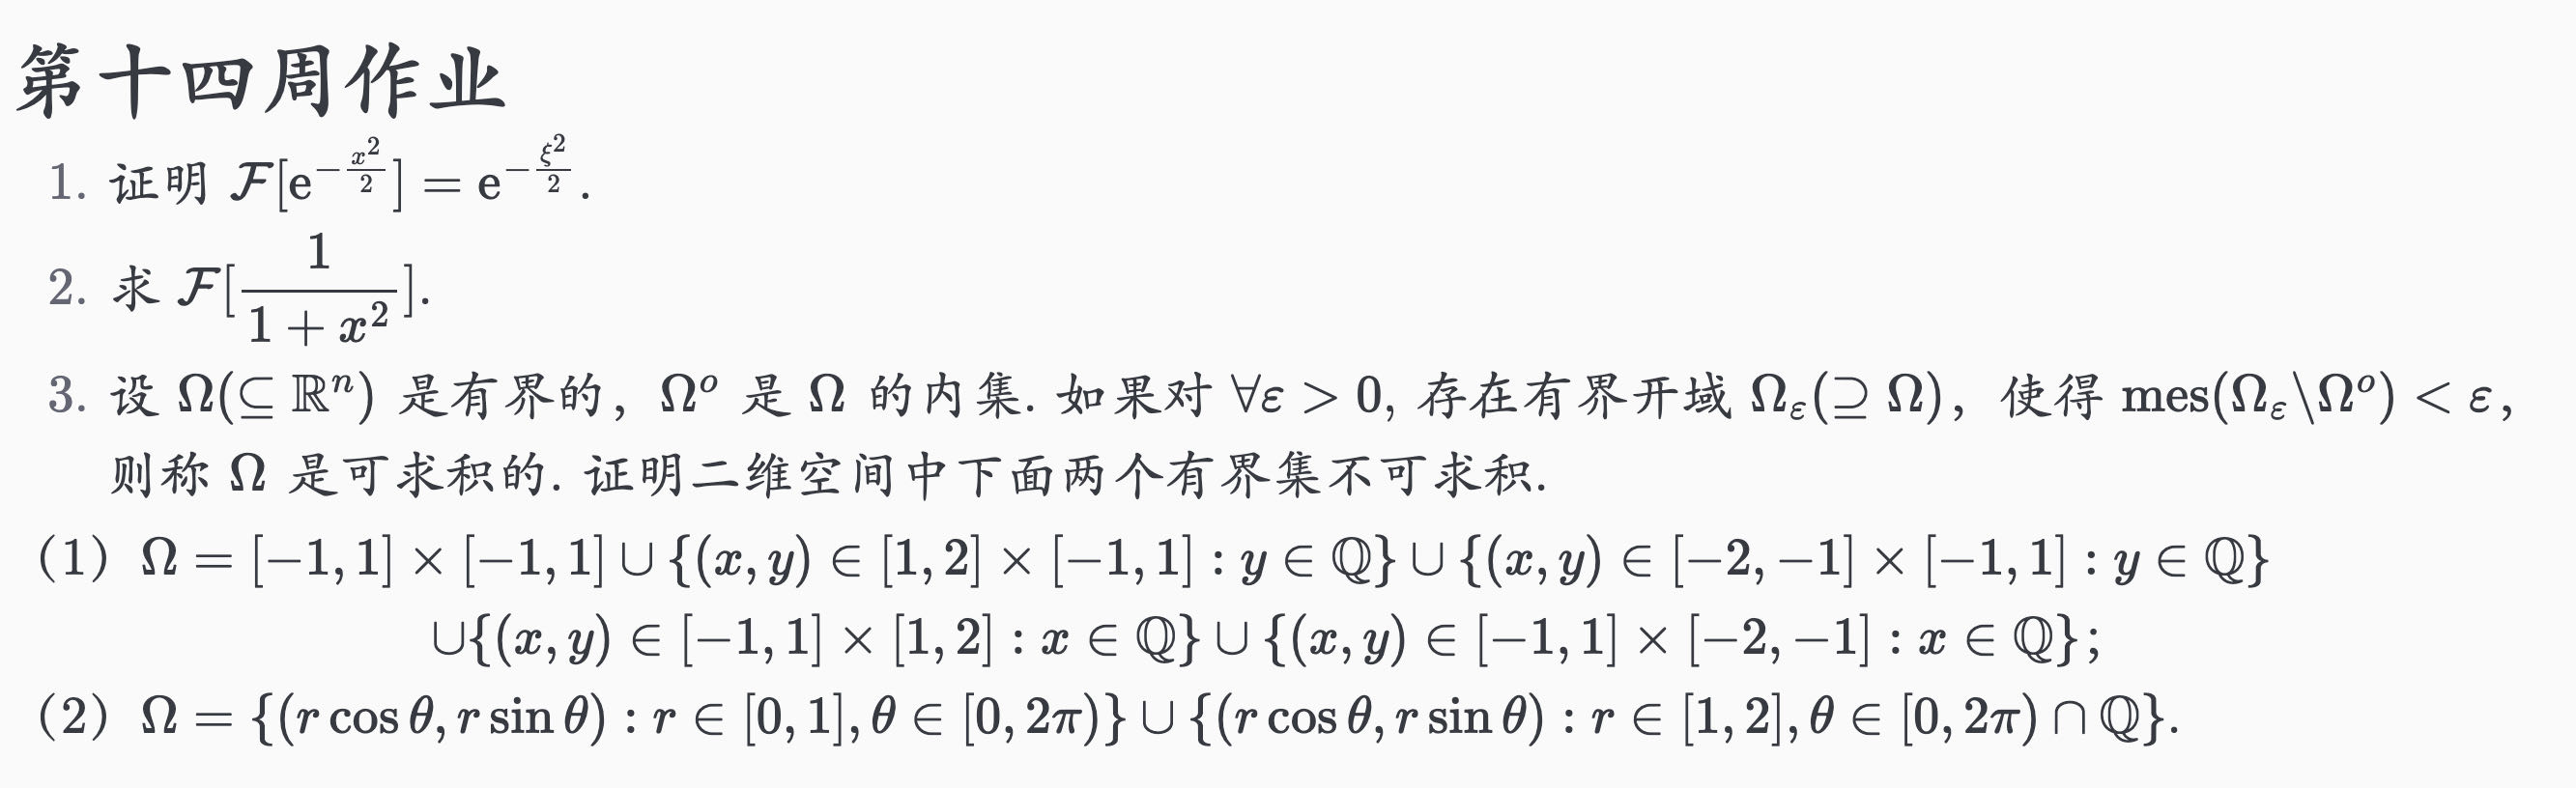
\includegraphics[width=\textwidth]{07d164620cb95c0559f2cea10ed3ec14.jpg}
% \caption{}
\label{}
\end{figure}

\begin{exercise}
证明:$\mathcal{F}\left[ e^{ -\frac{x^2}{2} } \right]=e^{ -\frac{\xi^{2}}{2} }$.
\end{exercise}
\begin{proof}
\[
\begin{aligned}
\mathcal{F}\left[ e^{ -\frac{x^2}{2} } \right] & =\frac{1}{\sqrt{ 2\pi }}\int_{-\infty}^{\infty} e^{ -\frac{x^2}{2} }e^{ -i\xi x } \, \mathrm{d}x \\
 & =\frac{1}{\sqrt{ 2\pi }}\int_{-\infty}^{\infty} e^{ -\frac{1}{2}(x+i\xi)^2 }\cdot e^{ -\frac{\xi^{2}}{2} } \, \mathrm{d}x  \\
 & =e^{ -\frac{\xi^{2}}{2} }
\end{aligned} 
\]
\end{proof}

\begin{exercise}
求 $\mathcal{F}\left[ \frac{1}{1+x^2} \right]$.
\end{exercise}
\begin{proof}
\[
\mathcal{F}\left[ \frac{1}{1+x^2} \right]=\frac{1}{\sqrt{ 2\pi }}\int_{-\infty}^{\infty} \frac{1}{1+x^2}e^{ -i\xi x } \, \mathrm{d}x
\]
Let $f (z)\coloneqq \frac{1}{1+z^2}e^{ -i\xi z }$. Consider the upper semicircle, we have
\[
\int_{-R}^{R} +\int_{\gamma_{R}^{+}} f(z)\, \mathrm{d}z =2\pi i\cdot \mathrm{res}_{i}f=2\pi i\cdot \lim_{ z \to i } \frac{1}{z+i}e^{ -i\xi z }=\pi e^{ \xi }
\]
\[
\left\lvert  \int_{\gamma_{R}^{+}}^{} f(z) \, \mathrm{d}z  \right\rvert  \leq \int_{\gamma_{R}^{+}}^{} \lvert f(z) \rvert  \, \lvert \mathrm{d}z \rvert  =\int_{0}^{\pi} \frac{1}{1+R^2e^{ i\cdot2\theta }}R \, \mathrm{d}\theta\to0\quad \text{as }R\to \infty 
\]
Thus
\[
\mathcal{F}\left[ \frac{1}{1+x^2} \right]=\frac{1}{\sqrt{ 2\pi }}\underbrace{ \int_{-\infty}^{\infty} \frac{1}{1+x^2}e^{ -i\xi x } \, \mathrm{d}x }_{ =\pi e^{ \xi } }=\sqrt{ \frac{\pi}{2} }e^{ \xi }
\]
\end{proof}

\begin{exercise}
\begin{figure}[H]
\centering
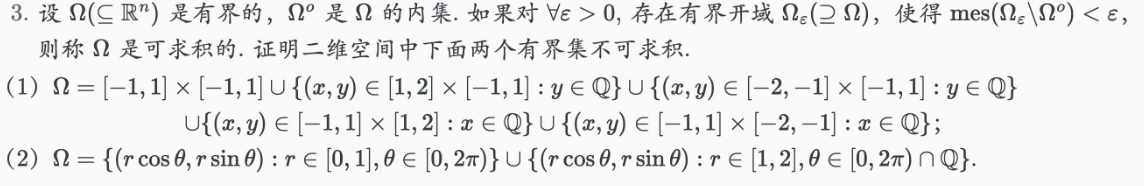
\includegraphics[width=\textwidth]{2-hw13-2025060317.png}
% \caption{}
\label{}
\end{figure}
补充:$\overline{\Omega}\subset \Omega_{\varepsilon}$.
\end{exercise}
First, we show that if $\Omega_{\varepsilon}$ is an open set containing $\Omega$ (and $\Omega$ is bounded), then $\bar{\Omega} \subseteq \Omega_{\varepsilon}$. Let $x \in \bar{\Omega}$. If $x \in \Omega$, then $x \in \Omega_{\varepsilon}$ since $\Omega \subseteq \Omega_{\varepsilon}$. If $x \in \bar{\Omega} \backslash \Omega$, then $x$ is a limit point of $\Omega$. Suppose $x \notin \Omega_{\varepsilon}$. Since $\Omega_{\varepsilon}$ is open, its complement $\Omega_{\varepsilon}^c$ is closed. Thus, if $x \in \Omega_{\varepsilon}^c$, there exists an $r>0$ such that the open ball $B(x, r) \subseteq \Omega_{\varepsilon}^c$, meaning $B(x, r) \cap \Omega_{\varepsilon}=\emptyset$. However, since $x$ is a limit point of $\Omega, B(x, r)$ must contain some point $y \in \Omega$. Since $\Omega \subseteq \Omega_{\varepsilon,} y \in \Omega_{\varepsilon}$. Thus $y \in$ $B(x, r) \cap \Omega_{\varepsilon}$, which contradicts $B(x, r) \cap \Omega_{\varepsilon}=\emptyset$. Therefore, $x$ must be in $\Omega_{\varepsilon}$. So, $\bar{\Omega} \subseteq \Omega_{\varepsilon}$.

(1)
Here we have $\Omega^{\circ}=[-1,1]\times[-1,1]$ and $\overline{\Omega}=[-2,2]\times[-1,1]\cup[-1,1]\times[-2,2]$. Then
\[
\text{mes}(\Omega_{\varepsilon}\setminus \Omega^{\circ })=\text{mes}(\overline{\Omega}\setminus \Omega^{\circ })=\text{mes}(\overline{\Omega})-\text{mes}(\Omega^{\circ })=8
\]
Since $\operatorname{mes}(\partial \Omega)=8 \neq 0$, the set $\Omega$ is not Jordan measurable.

(2)
Here we have $\Omega^{\circ}=\{ (r\cos\theta,r\sin \theta) :r\in[0,1],\theta\in[0,2\pi)\}$, and $\overline{\Omega}=\{ (r\cos\theta,r\sin\theta):r\in[0,2],\theta\in[0,2\pi) \}$. Then
\[
\text{mes}(\Omega_{\varepsilon}\setminus \Omega^{\circ })=\text{mes}(\overline{\Omega}\setminus \Omega^{\circ })=\text{mes}(\overline{\Omega})-\text{mes}(\Omega^{\circ })=4\pi-\pi=3\pi
\]
Since $\text{mes}(\partial \Omega)=3\pi\neq0$, the set $\Omega$ is not Jordan measurable.
